% author: Man Cao, Lilong Jiang
\documentclass{article}
\usepackage[letterpaper]{geometry} \usepackage[utf8]{inputenc}
\usepackage[T1]{fontenc}
\usepackage{amsmath}
\usepackage{hyperref}
\usepackage{relsize}
\usepackage{graphicx}
\usepackage{subcaption}

\newcommand{\code}[1]{\textsf{\smaller\verb~#1~}}

\begin{document}

\title{CSE5243 Assignment 5}
\author{Man Cao(cao.235), Lilong Jiang(jiang.573)}
\maketitle

\section{Work Separation}
Lilong mainly worked on part 1 of this project. Man mainly worked on
part 2. In fact there were a lot of overlapping during the
work, we exchanged various ideas and wrote the this report together.

\section{Software Used}
We use Orange \footnote{\url{http://orange.biolab.si}} to generate association
rules.
Orange implements the APRIORI algorithm to compute large itemsets and association
rules.

\section{Input}
After eliminating documents without topics, 11367 documents are left.\\
The input file has the following format:
\begin{verbatim}
{'NEWID':<value>, 'TOPICS':[value1, value2, ...], 'PLACES':[value1, value2, ...]}
{<term1>:<value1>, <term1>:<value2>, ...}
\end{verbatim}
Note that each document corresponds to two lines: the first line contains the
metadata of the document, the second line is the frequency vector.

\subsection{Data Transformation}
Orange supports transactional data input via the basket format. We first
transform our input to the basket format by dropping the <value> field in
the input file, then use Orange to generate association rules.
We convert the topics in an document to uppercase, and keep the terms in
the feature vector in lowercase, in order to easily separate them for later
processing.

\section{Algorithms}
We refer the algorithm in part 1 of this project as Alg 1, and the
algorithm with clustering in part 2 as Alg 2. For the clustering algorithm in
part 2, we use K-means.

\subsection{Handling Data Skew}
For Alg 1, we need to handle data skew in the training data, because there are
some topics that are dominant, and the rest of topics are rare. We first count
the number of documents for each topic, then find the first topic that accounts
for over 30\% of all documents. Second, we split the training data into two
parts: one contains the documents of the dominant topic, the other contains the
rest of documents. We generate association rules for the two parts separately,
then merge the two sets of rules and recompute support, confidence and lift for
each rule. In this way, we can reduce the impact of data skew on the associate
rule mining process.

\subsection{Sorting Criteria}
After trying out several sorting criteria, we decide to sort the rules
by [lift, confidence, support]. That is to first order rules by lift; then for
rules with same lift, order them by confidence; finally order rules with same
lift and confidence by support.

The reason behind our choice is that there are a lot of rules with
high confidence and support that only predicts one dominant topic. First sorting
by lift can make rules with good ability to predict rare topics
appear at the top of the list, so that they get a better chance to be used.

\subsection{Subsumption}
We use the following algorithm to determine rule subsumption:

Rule r1 is subsumption by rule r2 if all of the following conditions are
satisfied:
\begin{enumerate}
  \item r2 comes before r1 in the list of sorted rules.
  \item r1 can not predict any new topics compared to r2. That is: r1.right
  $\subseteq$ r2.right.
  \item all data instances that match r1 also match r2. That is:
  r1.match\_both $\subseteq$ r2.match\_both.
\end{enumerate}

\subsection{Accuracy for Multiple Topics}
To compute accuracy of classification in the presence of documents with
multiple topics, we use the following method:

$AC_d$ is the set of actual topics for document $d$; $PR_d$ is the set of
predicted topics for $d$; $DOC$ is the set of documents for testing. The
accuracy is:

\begin{equation}
\frac{\sum_{d \in DOC}\frac{|AC_d \cap PR_d|}{|AC_d|}}{|DOC|}
\end{equation}

In one word, we do not penalize accuracy if the predicted topics are more than
actual topics.

\section{Parameter Values}

\subsection{Minimum Support}
We have tested various values of minimum supports, and found out that the range
is pretty limited for Orange to generate rules on our data set. If
minimum support is less that 0.02, then there are too many frequent itemsets
that Orange cannot produce result; if it is more than 0.2, then Orange produces
no rule. Thus in the end we test with minimum supports of values 0.05, 0.1,
0.15.

\subsection{top-K rules}
We test with K = 1, 2, 3, 4, 5, to explore the impact of K for selecting top-K
rules in the sorted list of rules. We do not go beyond 5, according to the
discussion in class.

\subsection{Number of clusters}
We test with 8 clusters and 16 clusters, according to the description of the
project.

\section{Evaluation}

\subsection{Execution Time}

\begin{figure}
\centering
\includegraphics[width=0.8\textwidth]{buildmodel}
\caption{\footnotesize Time to build the model, i.e. to generate association
rules, for the two algorithms with different minimum supports. }
\label{Fig:buildmodel}
\end{figure}

\begin{figure}
\centering
\includegraphics[width=0.8\textwidth]{TestingTime1}
\caption{\footnotesize Time to run the model over the test data, for algorithm
1 with different minimum supports and K values. }
\label{Fig:TestTime1}
\end{figure}

\begin{figure}
\centering
\includegraphics[width=0.8\textwidth]{TestingTime2}
\caption{\footnotesize Time to run the model over the test data, for algorithm
2 with different minimum supports and K values. }
\label{Fig:TestTime2}
\end{figure}

\subsection{Quality}
\subsubsection{Accuracy}

\begin{figure}
\centering
\includegraphics[width=0.8\textwidth]{Accuracy}
\caption{\footnotesize The accuracy for the two algorithms with different
parameters. }
\label{Fig:Accuracy}
\end{figure}

\subsubsection{F-measure}
\begin{figure}
        \centering
        \begin{subfigure}[b]{0.4\textwidth}
         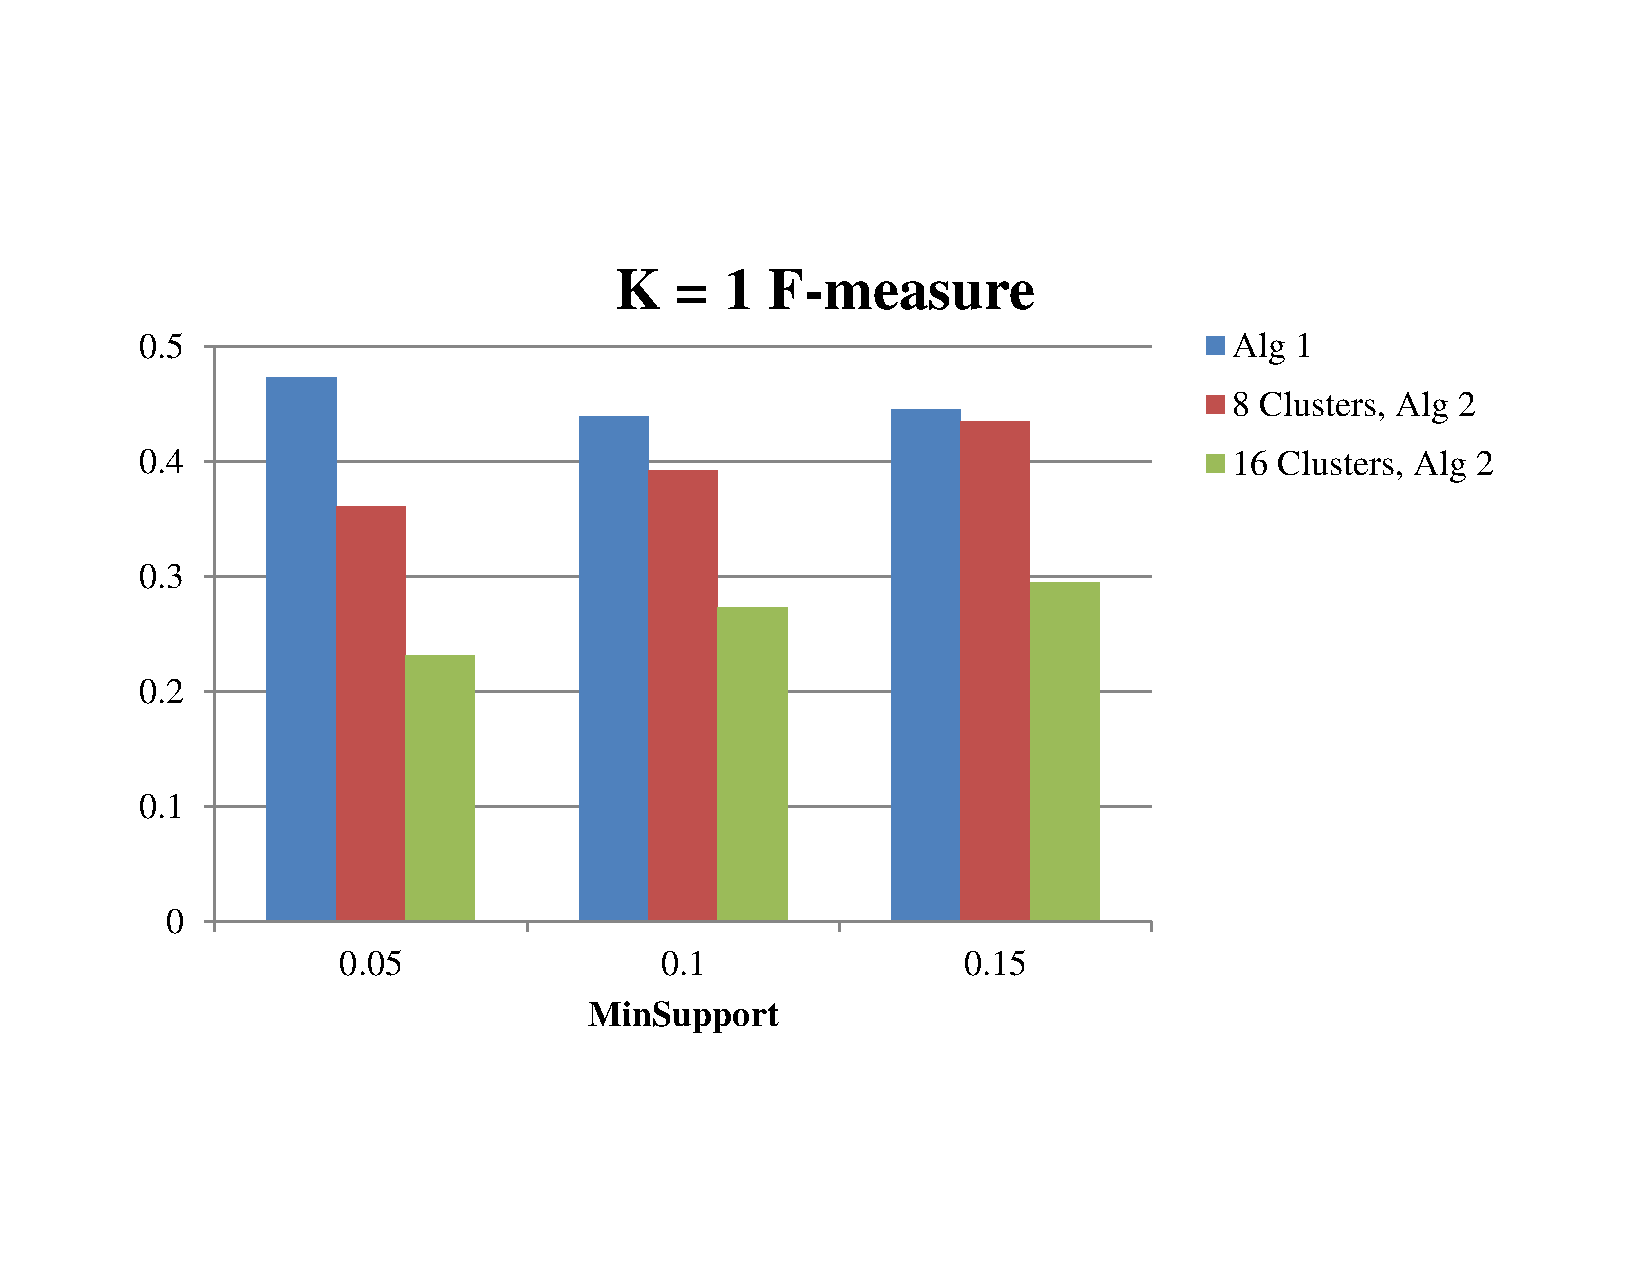
\includegraphics[width=\textwidth]{F-measure1}
         \caption{K = 1}
         \label{Fig:F-measure1}
        \end{subfigure}
        \begin{subfigure}[b]{0.4\textwidth}
         \includegraphics[width=\textwidth]{F-measure2}
         \caption{K = 2}
         \label{Fig:F-measure2}
        \end{subfigure}
        \begin{subfigure}[b]{0.4\textwidth}
         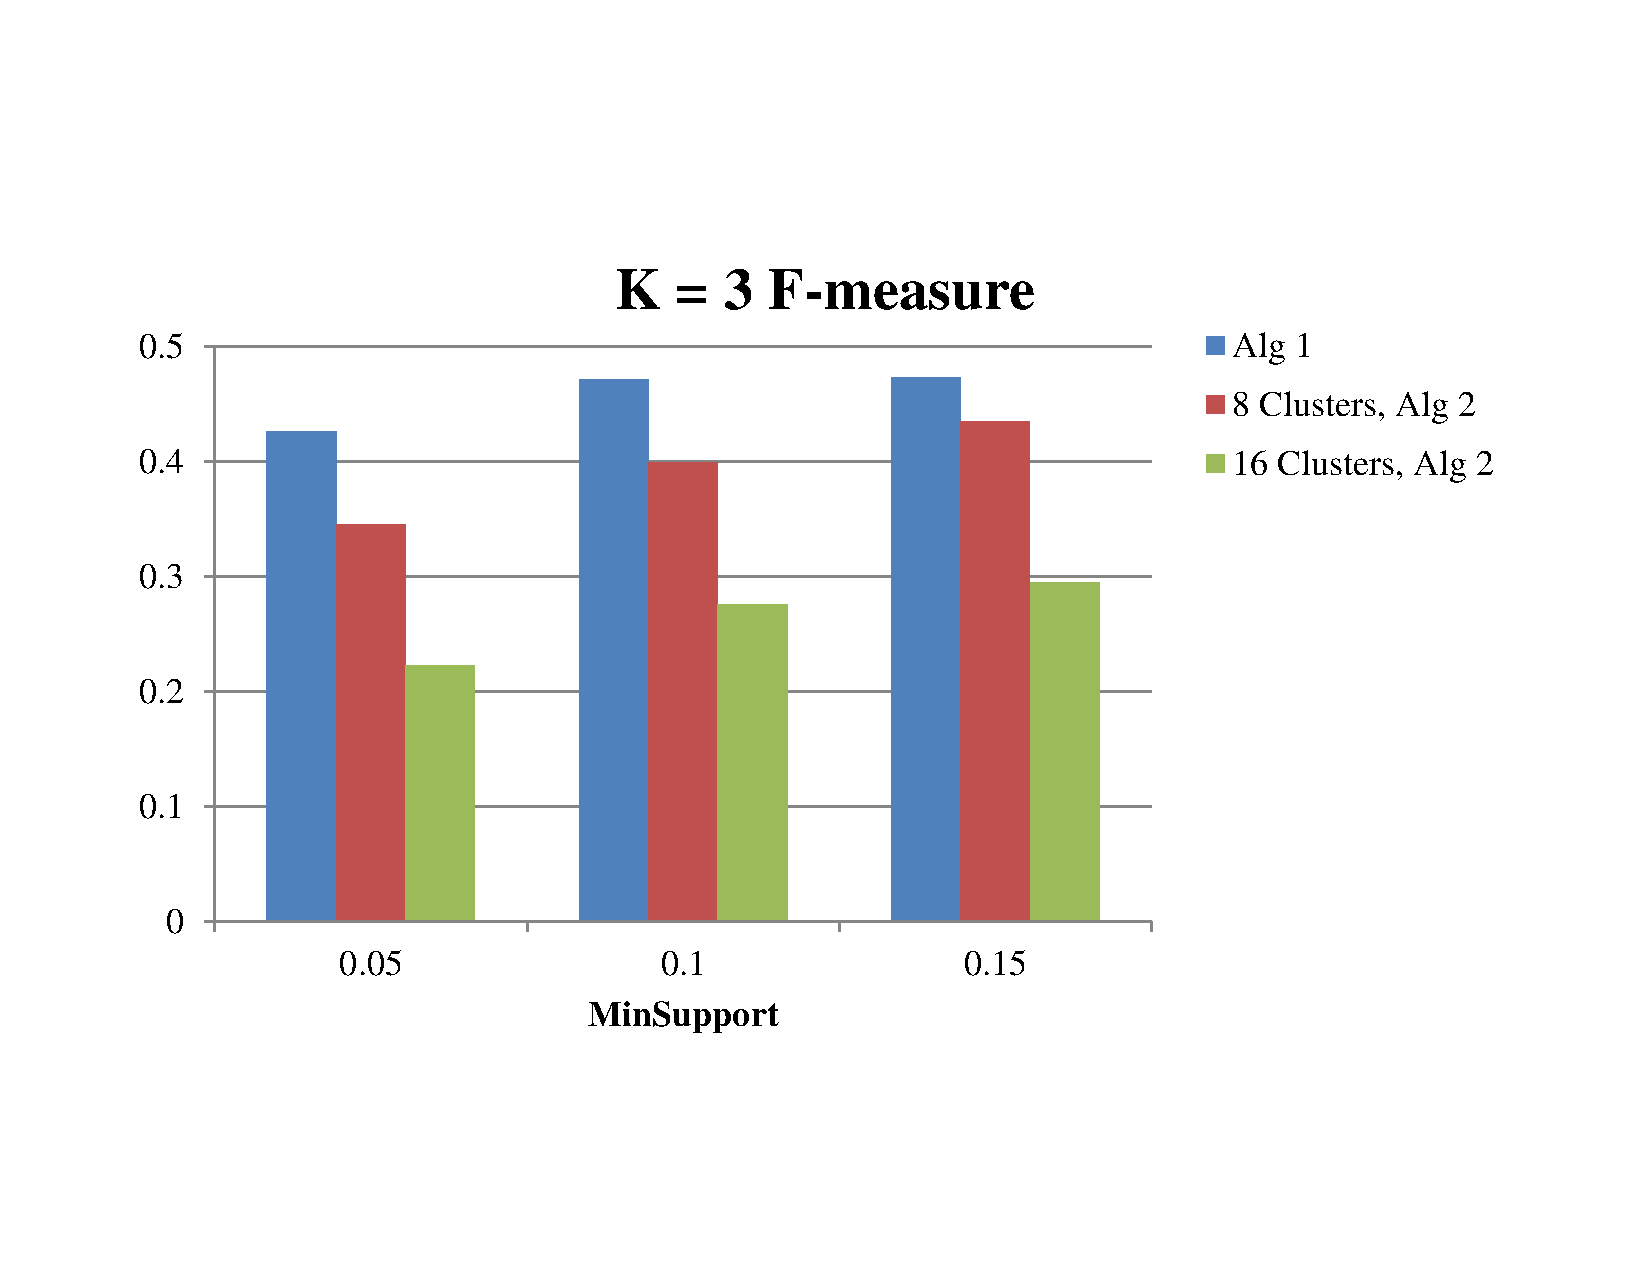
\includegraphics[width=\textwidth]{F-measure3}
         \caption{K = 3}
         \label{Fig:F-measure3}
        \end{subfigure}
        \begin{subfigure}[b]{0.4\textwidth}
         \includegraphics[width=\textwidth]{F-measure4}
         \caption{K = 4}
         \label{Fig:F-measure4}
        \end{subfigure}
        \begin{subfigure}[b]{0.4\textwidth}
         \includegraphics[width=\textwidth]{F-measure5}
         \caption{K = 5}
         \label{Fig:F-measure5}
        \end{subfigure}
        \caption{F-measures for two algorithms with different parameters.}
        \label{Fig:F-measure}
\end{figure}

\subsubsection{Skew}


\end{document}
